Elérkeztünk a \textit{GTK} egyik legrugalmasabb, legszélesebb körű funkciókkal felruházható, ugyanakkor  legkomplexebb eszközéhez. A \textit{widget}, objektumok együtteseként egyszerre teszi lehetővé az adatok megjelenítését, bevitelét, az elemek kiválasztást, keresését, szűrését, rendezését. Alapvető funkciója azonos típusú objektumok tulajdonságainak táblázatos formában történő megjelenítése, illetve kezelése, ahol a sorok az egyes objektumokhoz reprezentálják, míg az oszlopok az objektum egy adott tulajdonságához tartoznak.

\section{Fogalmak}

\subsection{Modell-nézet-vezérlő}

A \textit{widget} működése a modell-nézet-vezérlő elvet követi, vagyis elválik egymástól az adatok tárolására, illetve megjelenítésére, valamint vezérlésére szolgáló réteg. Ez egyfelől rugalmasságot tesz lehetővé a működés tekintetében, a performancia javulását is eredményezheti kellő körültekintés mellett, ugyanakkor sajnálatos módon bonyolítja az implementációt. Az eddigiekben is találkoztunk már ezt a mintát követő \textit{widget}ekkel (\texttt{GtkEntry}, \texttt{GtkComboBoxText}) ugyanakkor ezen \textit{widget}ek esetén a háttérben ugyan ez a minta húzódik meg, de használat során ennek hatásait elkerülhetjük. Ez esetben azonban a nézet és a modell elválasztása kötelező és nem megkerülhető.

\subsection{Modell}

A modell-nézet-vezérlő mintában a modell jelenti adattároló réteget, a \textit{GTK} terminológia ettől némiképpen eltér. A modell egy absztrakt osztály, ami a nézet irányába történő adatszolgáltatáshoz szükséges függvényeket, illetve szignálokat írja le. A tényleges adattárolóknak ezen absztrakt osztályt kell megvalósítaniuk, vagyis saját belső adatreprezentációjukat elrejtve a külvilág -- ez esetben a nézetet megvalósító \textit{widget} -- felé a modell által definiáltak megfelelően kell működniük. A \textit{GTK} a modell két implementációját is biztosítja, egyet a lista, egyet a fa szerkezettel rendelkező adatokhoz számára, ezzel együtt természetesen ha a saját adattárolónkat tartjuk performancia vagy egyéb okoknál fogva alkalmasabbnak, azt minden további nélkül használhatjuk, ha teljesítjük a modell által leírtakat.

\subsection{Nézet}

A nézet (\textit{view}) a megjelentő réteg a modell-nézet-vezérlő mintában. A modellben tárolt adatokat, valamint az adatok változását jelző szignálokat felhasználva végzi adatok megjelenítését, számos, az adatok típusára, formátumára vonatkozó paraméternek megfelelően. Maga a nézet alakítja ki a táblázatos megjelenési formát, annak oszlopaival és soraival, az ezek metszéspontjaiban található cellákkal, kezelve a megjelenítéskor azt a helyzetet, hogy a modellben tárolt adatok mennyisége többszöröse lehet annak, amit a nézet egy időben megjeleníteni képes. Egy modellhez több nézet is rendelhető, vagyis ugyanazon adatok több különböző formában jeleníthetjük meg. Ez jelentheti például, hogy más-más modellbeli oszlopok megjelenítése történik, más sorrendben, vagy más szűrésnek megfelelően, esetlen más szövegformázási paraméter mellett.

\subsection{Elemek elérése}

Maga a modell definiálja az adattároló elemeihez -- sorok és ezen belül cellák -- hozzáférését, illetve az adattároló elemeinek bejárását lehetővé tevő eszközöket, illetve módszereket. Három funkciójában eltérő eszköz is rendelkezésünkre áll az adattároló egyes elemire való hivatkozásra. 

\paragraph{Bejáró}

Az első és egyben a leggyakrabban használt ezek közül a bejáró (\textit{iterator}), ami az adattároló egy eleméhez -- legyen az lista vagy fa -- ad hozzáférést. A bejáró, mint a bejárók általánosságban, az adott elemre (itt sor) nézve csak akkor bír érvényes hivatkozással, ha az adattároló szerkezetében változatlan. Egyszerűbben fogalmazva egy bejáró csak addig érvényes, amíg az adattárolóhoz újabb elemet nem adunk (amivel egyébiránt újabb bejáró jön létre), vagy veszünk el belőle. A bejárón keresztül közvetlenül írhatjuk vagy olvashatjuk a vonatkozó sor egyes elemeit, celláit, ami természetesen a szerkezetet nem érinti, így sem a hozzáférést biztosító sem más bejárókat nem érvénytelenít. A bejárók mint látható erősen kötődnek a hivatkozott adattárolóhoz, egy adott modellre vonatkozó bejáró más modell esetén nem használható fel.

\paragraph{Útvonal}

A modell egy eleme megadható a modellben elfoglalt pozíciójával is, ezt teszi az útvonal (\textit{path}) leírására szolgáló objektum. A modellben elfoglalt pozíció szó szerint az jelenti, hogy az adott elem hányadik az eleme sorában, a \textit{C} nyelvi hagyományoknak megfelelően nullától kezdve a számlálást. Ha nem listában, hanem fában gondolkodunk, akkor ez annyi elemet jelent amilyen mélyen (\textit{depth}) az adott sor elhelyezkedik a fában. Az elem sorozata pedig a fa gyökerétől indulva az adott részfában a sor indexe.

\begin{figure}[h]
\begin{center}
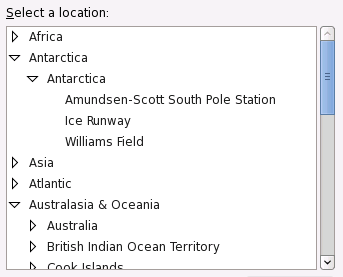
\includegraphics[width=50mm]{images/tree.png}
\caption{Útvonal fa szerkezeten belül\cite{gnomehig}}
\end{center}
\end{figure}

Az ábrán a \textit{William Field} értéket tartalmazó sor útvonalát az $1, 0, 2$ sorozat írja le, hiszen a legfelső szinten lévő második elem, első gyerekének, harmadik gyermeke. Az útvonal nem kötődik a modellhez, így egy útvonal bármelyik modellel együtt értelmezhető. Ha az útvonal létezik akkor visszakaphatjuk az mutatott sorhoz tartozó bejárót, amin keresztül már hozzáférhetünk az adatokhoz. Mivel nincs kötődés a modellel maga az útvonal objektum mindig érvényes, csak egy adott modell esetén nem garantált, hogy az útvonalon található sor.

\paragraph{Referencia}

A referencia (\textit{row reference}) olyan hivatkozás az adattároló egy sorára, ami mindaddig érvényes marad, amíg maga a sor létezik. A bejáróval ellentétben tehát hiába változik az adattároló szerkezete -- hozzáadás, vagy törlés révén -- a referencia érvényes marad, eltekintve attól ha épp az adott sort (is) töröltük. A referencia hasonlóan a bejáróhoz kötődik az adattárolóhoz, csak egy adott modellen érvényes. Az érvényesség lekérdezhető, az objektum mind útvonallá, mind pedig bejáróvá átalakítható. Ez utóbbi révén a modell adataihoz való hozzáférés is biztosított.

\section{Alapműveletek}

\subsection{Létrehozás}

\subsubsection{Modell}

A \textit{GTK} által implementált -- listák kezelésére használható -- adattároló (\texttt{GtkListStore}) legegyszerűbben úgy képzelhető el, mint egy táblázat. Ezen táblázat alapvetése, hogy egyforma típusú elemek megjelenítésére szolgál, legyenek azok fájlok, elektronikus levelek, vagy tűzfalszabályok. Az egyes sorokban az egyes elemek tulajdonságai szerepelnek, következésképp minden oszlop típusa azonos, amik soronként eltérő értékeket vesznek fel.

Ennek megfelelően a létrehozás során nem kell mást tennünk, mint megadnunk az oszlopok számosságát, illetve az egyes oszlopok típusát. Ez lényegében nem jelent komoly feladatot, ugyanakkor viszont ez egyes nyelvi változatok között komoly eltérések tapasztalhatóak, ami leginkább a nyelvi sajátosságoknak köszönhetőek.

\lsttriplesource
[numbers=none]
{sources/list_store_create.h}
{sources/list_store_create.hpp}
{sources/list_store_create.py}
{\texttt{GtkListStore} létrehozása}
{lst:liststorecreate}

Ahogy látszik a (\textit{C} nyelvi változat elvárja tőlünk, hogy megadjuk hány oszlopa lesz az elkészítendő adattárolónknak (\textit{store}). A változó hosszúságú paraméterlistájú függvénynél csak akkor van módunk rájönni, hogy mikor van vége a típusok felsorolásának, ha van olyan érték, amit a \texttt{GType} típus elemei nem vesznek fel. Hasonló a helyzet az átadott tömb kapcsán is. Így viszont nem marad más választásunk mint az oszlopok számát előre közölni. A másik két nyelvi változat kézenfekvő módszereket ad egy konténer méretének, illetve az átadott paraméterek számának lekérdezésére így annak külön megadására explicit módon nincs szükség.

\index{referencia-számlálás}
\index{lebegő referencia@''lebegő'' referencia}
\index{GObject@\texttt{GObject}!függvények!unref@\texttt{unref}} 
Külön említést érdemel a függvények visszatérési értéke, azaz az adattároló nyelvi változatnak megfelelő reprezentációja. Mindhárom esetben igaz, hogy a visszakapott érték egy referencia-számlált objektumok, lévén a \texttt{GtkListStore} a \texttt{GObject} típusból származik, viszont ez az egyes nyelveken különböző módokon jelenik meg. A \textit{C} változat egy mutatóval tér vissza, ahogy az szokás a \textit{widget}ek esetén is, a különbség mindössze annyi, hogy a specifikus típusra kapunk mutatót, ahogy ez a többi \texttt{GObject} típusból származó osztály esetén is igaz lesz. Itt a referencia növelése csak akkor történik meg, ha azt explicit módon kérjük, vagy azt adattárolóval hívott objektum -- például a nézet -- maga megteszi. A \textit{C++} változat egy intelligens mutatóval (\textit{smart pointer}) tér vissza, ami másolásakor implicit módon maga biztosítja a referenciaszám növelését, így ezzel nekünk nem kell törődnünk. A \textit{Python} nyelvi szinten rendelkezik referencia-számlálási megoldással, így itt nem szükséges az objektumok allokációjának és felszabadításának részleteivel törődnünk.

A referencia-számlálás már csak azért is fontos, mert egy modellre több nézetet is csatolhatunk, amiknek egyenként növelik a referencia értékét, hogy biztosítsák az adattároló objektum fennmaradását addig, amíg a nézet ezt használja. Az adattároló nem \textit{widget}, vagyis az alapfogalmak között említett ''lebegő'' referencia szerinti működés itt nincs érvényben, azaz az adattároló referenciaszámának értéke egy lesz létrehozáskor és már ez első nézet modellhez való csatlakoztatása azt eredményezi, hogy referenciaszám eggyel nő. Következésképp tehát minden csatolt nézet megszűnése után az adattároló referenciaszámának értéke újra egy lesz, tehát az nem szűnik meg automatikusan. Ha azt szeretnénk, hogy a modell a nézetek megszűntével maga is megszűnjön, akkor az nézet(ek) csatolása után csökkentenünk kell a referencia értékét. Mivel a referencia-számlálás funkcióját a \texttt{GObject} típus adja, ennek \texttt{unref} függvényét kell hívnunk.

\lsttriplesource
[numbers=none]
{sources/list_store_create_example.c}
{sources/list_store_create_example.cc}
{sources/list_store_create_example.py}
{Példa \texttt{GtkListStore} létrehozására}
{lst:liststorecreate}

A gyakorlatban minden nyelvi változat kapcsán kialakult a nyelv sajátosságaihoz idomuló módszer, amivel a későbbiekben a tároló könnyel kezelhetővé válik, aminek alapjait értelemszerűen a létrehozáskor tesszük le.

A \textit{C} nyelvi változat esetén egy sorszámozott típus (\texttt{enum}) tud rajtunk leginkább segíteni, ahol a típus egyes elemeinek nevei utalnak funkciójukra. Az előtagként használhatunk a tárolóra utaló (pl: \texttt{STORE\_NAMES}) szöveget, majd folytathatjuk a \texttt{COL} rövidítéssel, ami az érték oszlopsorszám mivoltát jelenti, míg az utótag az oszlopban tárolt adatra vonatkozhat. Ezzel olyan nevet kapunk, amit a későbbiekben a tárolóba való írás, illetve az onnan való olvasás esetén öndokumentálóvá teszi a kódot, ellentétben a puszta sorszámokkal, amik \textit{magic number}ként jelennek meg a kódban.

A \textit{C++} változat maga szolgál egy osztállyal (\texttt{TreeModel::ColumnRecord}) ami az oszlopok leírására szolgált. A gyakorlatban származtatás révén érjük el, hogy tároló konstruktora az épp elkészítendő objektumra specifikus oszlopleírót kaphasson. Ebben a származtatott osztályban nincs más dolgunk -- ahogy az a példában is látszik --, mint publikus tagként -- mivel a későbbiekben ezen objektum adattagjait használjuk az írás, olvasás műveletnél az oszlopok azonosítására -- felsorolni és ezeket a konstruktorban hozzáadni az objektum privát konténeréhez (\texttt{add}). Ezen konténer lekérdezhető a \texttt{size} függvénnyel, aminek révén a tároló is tudni fogja voltaképpen hány oszloppal is rendelkezünk.

A \textit{Python} változat újfent a legegyszerűbb, de legalábbis a legrövidebb, így bizonyos értelemben ezzel járunk a legjobban. Újdonságot a másik két változathoz képest nem tartalmaz, megjegyezni is csak annyit érdemes vele kapcsolatban, hogy az oszlopokhoz használt saját osztály helyett ha származtatunk a \texttt{GtkListStore} típusból, akkor azon belül definiálhatjuk a névvel azonosított oszlopsorszámokat. A \textit{C} változathoz hasonlóan itt is érdemes különös figyelmet fordítani arra, hogy az oszlopok sorszámai és a típusok helyes sorrendben legyenek, különben futás közben váratlan és nehezen visszanyomozható hibákba ütközhetünk.

\subsubsection{Nézet}

A nézet (\textit{view}) létrehozása önmagában egy rendkívül egyszerű feladat, hiszen akár paraméter nélkül is létrehozható, vagy paraméterként átadható egy modell is, ami természetesen később is beállíthatunk a nézetnek (\texttt{set\_model}).

\lsttriplesource
[numbers=none]
{sources/tree_view_create.h}
{sources/tree_view_create.hpp}
{sources/tree_view_create.py}
{\texttt{GtkTreeView} létrehozása}
{lst:treeviewcreate}

A teljes modell-nézet-vezérlő szerkezet nézet részének csak egy része maga a \texttt{GtkTreeView}, ugyanakkor a feladat érdemi részét nem ez, hanem az oszlopok hozzáadása jelenti. Amint az a modell felépítéséből következik, az oszlopok azonos típusú értékeket tartalmaznak, tehát azonos eszközzel is kell őket megjelenítenünk. Ez az eszköz az oszlop -- a hozzá tartozó osztály pedig a \texttt{GtkTreeViewColumn} --, ami gondoskodik az oszlop, illetve fejlécének megjelenítéséről, az oszlop átméretezhetőségéről, nem gondoskodik azonban a sorok és oszlopok metszéspontjaként adódó cellák megjelenítéséről, ezt egy külön osztály végzi.

\lsttriplesource
[numbers=none]
{sources/tree_view_column_create.h}
{sources/tree_view_column_create.hpp}
{sources/tree_view_column_create.py}
{\texttt{GtkTreeViewColumn} létrehozása}
{lst:treeviewcolumncreate}

Ahogy látszik \texttt{GtkTreeViewColumn} létrehozható akár paraméterek megadása nélkül is, bár ennek csak akkor van értelme ha a létrehozást követően adjuk meg a paramétereket, amikre a létrehozáskor is lehetőségünk lett volna. Az oszlop kapcsán kézenfekvő, hogy meg kell adnunk az oszlop fejlécének szövegét (\texttt{title}), az objektumot, ami a cella kirajzolását végzi majd (\textit{renderer}), illetve ennek paramétereit, amik közül messze a legfontosabb, hogy a modell melyik oszlopában található az adat, aminek a képernyőn való megjelenítése a feladata lesz.

Az iménti példában látott paraméterezéssekkel az egyes nyelvi változatokban léteznek függvények (\texttt{insert\_column}, \texttt{insert\_column\_with\_attributes}), amik egyrészt elkészítik a \texttt{GtkTreeViewColumn}, illetve \texttt{GtkCellRenderer} objektumokat, majd az oszlopot hozzá is adják nézethez, az első paraméterként megadott pozícióra. Az oszlopok sorrendje a hozzáadás révén meghatározottá már válik, hiszen az egymás után a nézethez hozzáadott (\texttt{append\_column}) oszlopok -- hasonlóan a konténerekbe helyezett \textit{widget}ekhez -- egymás mellett, balról jobbra helyezkednek majd el, a beszúrt oszlopoknál (\texttt{insert\_column}) a helyet egy kötelezően megadandó paraméter határozza meg.

\lsttriplesource
[numbers=none]
{sources/tree_view_create_example.c}
{sources/tree_view_create_example.cc}
{sources/tree_view_create_example.py}
{Példa \texttt{GtkTreeView} létrehozására}
{lst:treeviewcreate}

Az oszlopok hozzáadásának két fontos kérdését segít tisztázni a fenti példa. Az egyik az oszlop pozíciója. Mint arról szó esett az \texttt{append\_column} függvény minden eseteben az eddigi oszlopok után fűzi az új oszlopot, ahogy ez a nevéből is következik, míg az \texttt{insert\_column} a megadott pozícióra szúrja be az új oszlopot, kivéve ha a pozíció $-1$, mert ez esetben az \texttt{append\_column} függvénnyel azonos módon működik. Visszatérési értékük az új oszlop pozíciója ami alapján később a nézet vissza tudja adni nekünk az oszlopot. Elkerülendő, hogy ez érték kompromittálódjon, célszerű az oszlopokat mindig a sor végére hozzáfűzni.

A másik kérdés, hogy miként szerez tudomást róla a \texttt{GtkCellRenderer} objektum, hogy honnan szerzendő be a megjelenítendő adat, illetve mik lennének annak megjelenítési paraméterei. Az \texttt{append\_column}, illetve az \texttt{insert\_column} függvényeknek átadott utolsó két paraméter nem az oszlopnak, hanem a \texttt{GtkCellRenderer} objektumnak szóló paraméterek és azt mondják meg, hogy a létrejött \texttt{GtkCellRendererText} objektum az egyes sorok esetén az adattárló mely oszlopából vegye a saját \texttt{text} paraméterének értékét. Nem meglepő módon a \texttt{GtkCellRendererText} objektum a \texttt{text} attribútumának értékét jeleníti meg a sor és az oszlop által meghatározott cellában. Ez a működési modell nem csak azt teszi lehetővé, hogy a megjelenítendő szöveget adjuk meg a modell valamelyik oszlopában -- ami egyrészről értelemszerű, másrészről a működéshez elégedetlen is -- de például annak előtét-, vagy háttérszínét (\texttt{foreground}, \texttt{background}) is.

\subsection{Kezelés}

\subsubsection{Modell}

\paragraph{Hozzáadás}

Az adattároló feltöltésének első lépése az új sor beszúrása a megfelelő helyre. Ennek legegyszerűbb módja az, ha az eddigi elemek mögé egy új elemet szúrunk be. Ez minden további nélkül megtehető az adattároló (\textit{store})\footnote{megjegyzendő, hogy az elem hozzáadását nem a modell definiálja, ez csak olvasáshoz ad interfészt} bejárót visszaadó \texttt{append} függvényével. Természetesen éppúgy lehetőség van a meglévő elemek elé (\texttt{prepend}), vagy adott pontra történő beszúrására (\texttt{insert}), bár ezek gyakorlati jelentősége kisebb. Fák esetén ugyanezen függvények ugyanúgy léteznek, egy eltéréssel. Ez pedig az, hogy a első paraméterként a szülő elemhez tartozó bejárót kell megadni, illetve ha legfelső szintű elemet szeretnénk, akkor a nyelvi változatnak megfelelő \textit{null} értéket kell átadni.

\lsttriplesource
[numbers=none]
{sources/list_store_append.h}
{sources/list_store_append.hpp}
{sources/list_store_append.py}
{Elem hozzáadása listához}
{lst:liststoreappend}

\lsttriplesource
[numbers=none]
{sources/tree_store_append.h}
{sources/tree_store_append.hpp}
{sources/tree_store_append.py}
{Elem hozzáadása fához}
{lst:liststoreappend}

A különbség ez egyes nyelvek között talán nem látványos, de egy ponton mindenképpen számottevő. A \textit{C++}, illetve \textit{Python} nyelvű megvalósítás az új bejárót visszaadja, míg a \textit{C} megoldásában egy kimeneti paraméterben kapjuk vissza. Ez elsőre csak formai eltérésnek tűnhet, de ettől mélyebb oka van. Az előbbi két nyelv esetén a bejárok objektumok, míg az utóbbi nyelv esetében -- lévén erről nem lehet szó -- mindössze egy struktúra. Az paraméterként elvárt mutató -- kimeneti paraméterről lévén szó -- egy létező bejáró struktúrára kell mutasson, amit az \texttt{append}, \texttt{insert\_before} és egyéb függvények töltenek ki a megfelelő értékekkel, amit ezt követően vehetünk az adatok eléréséhez használatba.

\paragraph{Feltöltés}

Az elem hozzáadására használt függvények deklarációjából látszik, hogy a \textit{Python} nyelv esetén lehetőség van egy lépésben hozzáadni egy új elemet az adattárolóhoz és egyszersmind megadni az új sor egyes oszlopokba eső értékeit, a \texttt{row} paraméter révén. A \texttt{C} illetve \texttt{C++} változat ezt két lépésben végzi, először hozzáadja az új elemet az adattárolóhoz, mahd csak ezt követően ad értéket a celláknak. Ez nem teljesen fedi a valóságot, mivel a \textit{C} nyelv esetén is van mód az egy lépéses megoldásra, ami nem is meglepő, hiszen a \textit{Python} változatban sem lenne különben erre lehetőség. A \textit{C} nyelvi függvény neve \texttt{insert\_with\_values}, ami paraméterezését tekintve összefűzése az \texttt{insert} és a feltöltésre szolgáló \texttt{set} függvényekének. A \texttt{C++} esetén a valóság megegyezik a látszattal, vagyis csak a két lépcsős megoldás létezik, ami járhat némi hatékonyságproblémával, de még ettől is bonyolultabb a helyzet némiképp.

\lsttriplesource
[numbers=none]
{sources/store_set.h}
{sources/store_set.hpp}
{sources/store_set.py}
{Elem hozzáadása fához}
{lst:storeset}

\paragraph{Lekérdezés}

\paragraph{Bejárás}

\subsection{Szignálok}

\subsubsection{Vezérlő}

\section{Tesztelés}

\subsection{Típusok}
\subsection{Állapotok}
\subsection{Műveletek}
\subsection{Interfészek}
